\newpage{}
\section{Materials and Methods}

% Add small intro here 
This section gives an overview about the dataset used for classification, as 
well as a conceptual overview of the experimental setup and the assumptions 
behind that setup. For a source-code 
focused view of the project, refer to Section~\ref{sec:implementation}.

\subsection{Dataset}\label{sec:materials_dataset}

Though this thesis treats the analysis of a set of \ac{mri} scans, these scans
were not produced by the author. The dataset was provided % TODO:
by the Institute of Radiology % TODO: Don't forget new scans
of the \ac{salk}. It consists of \ac{mri} scans of 102 patients, where 24 reached 
\ac{pcr}. Due to mismatches in geometry between annotation and scan, 9 scans
could not be used. This leaves 93 patients, 22, or \SI{23.366}{\percent}, of which achieved 
\ac{pcr}. All scans were manually annotated.

The dataset may not be published, as it underlies an obligation of anonymity to 
the patients the scans were recorded of. Additional available metadata to that 
mentioned above is listed in the appendix under Section~\ref{sec:mri_metadata}.

The exact definition of \ac{pcr} is not always clear or consistent.
In this context, it signifies absence of cancer tissue
around the site of occurrence after treatment. This includes \enquote{[\dots] 
the total absence of neoplastic cells [tumors] in the rectal wall, mesorectum, 
and mesorectal lymph nodes}~\cite[p.~2823]{Zorcolo2012}\cite{clinical_and_oncological_results_of_pcr}.
% TODO: Describe metadata, maybe add table in appendix?
% TODO: Who annotated the dataset - Kinda done

The dataset is not annotated consistently; most scans contain a 2-dimensional 
annotation, marking a slice of tumor, while \threeDcount{} scans are annotated along all 
three axes. To avoid inconsistencies, all annotations were interpolated to form
a 3-dimensional annotation from their largest slice, as described 
in~\ref{sec:3d_and_2d}.

\subsection{Choice of Tools}

As is popular with machine learning projects, this program is implemented in 
Python\footnote{\hyperlink{https://www.python.org/}{More information available 
at https://www.python.org/}.}. It offers the possibility of quick prototyping, 
intuitive and easily readable syntax and, most importantly, a large tool set for
both radiomics and machine learning applications. 

To address the earlier mentioned problem with the definition and extraction of
radiomics features, a widely available and well documented library was chosen.
PyRadiomics\footnote{More information available at 
\hyperlink{https://www.radiomics.io/pyradiomics.html}
{https://www.radiomics.io/pyradiomics.html}.\\Documentation available at 
\hyperlink{https://pyradiomics.readthedocs.io/en/latest/}
{https://pyradiomics.readthedocs.io/en/latest/}.} covers, and is compatible to,
most features defined by the \ac{ibsi}, while documenting any differences in 
features definition or calculation (such as correcting for negative values, 
which may not be covered in the \ac{ibsi} formula).
Additionally, PyRadiomics offers tools to pre-process data, e.g.~normalization
of input images or passing input images through predetermined filters.

Next, the features extracted by PyRadiomics have to be processed. In the context
of this project, this means to classify an input image into two categories: 
expected \enquote{\ac{pcr}} or \enquote{non-\ac{pcr}}. As discussed earlier, % TODO: make sure to discuss this earlier
a random forest classifier was chosen for this task. The toolkit used to 
implement this classification model is \texttt{sklearn}, which offers an 
implementation of a random forest classifier through
its \\\texttt{sklearn.ensemble.RandomForestClassifier} class. It offers an
accessible and easy to use interface and compatibility with other feature-rich
data analysis tools (such as, but not limited to, \texttt{numpy}, 
\texttt{pandas} and \texttt{matplotlib}). Additionally, being an open-source
project, the library is both cheap (i.e.~free) to acquire and use 
(assuming no license violations) and easy to version and distribute, increasing 
reproducibility. 

As a connection between extraction and classification and analysis of results, a
multitude of other libraries are required. Though important in their own rights,
these libraries are not of special interest in the context of this thesis and 
will be addressed when relevant, instead of introducing them here.

\subsection{Experimental Setup}\label{sec:experimental_setup}

% Short summary of what I do

As stated earlier, this thesis aims to determine, if \ac{pcr} of a colorectal
tumor patient can be predicted through a radiomics-based classification model,
using \ac{mri} scans as input. To be considered successful, the model has 
to achieve a (balanced\footnote{Unless explicitly
stated otherwise, all mentions of \enquote{accuracy} refer to \enquote{balanced
accuracy}.}) accuracy deviating significantly from 0.5, or \SI{50}{\percent}. 

The model chosen is \iac{rf} classifier. The model is trained on a set composed
of \SI{70}{\percent} of all \ac{pcr} patients and an equal amount of non-\ac{pcr} patients,
both chosen randomly. The testing set consists of all remaining patients.
Each patient is represented by \iac{mri} scan accompanied by an annotation 
marking the contained tumor. Before feature extraction, this annotation is 
passed through a common extrapolation algorithm to create a 3-dimensional 
\ac{roi}. From this, radiomics features are extracted using PyRadiomics. A 
common extractor is used for all patients; its configuration file can be found
in the appendix under Listing~\ref{code:pyrad_config}. The majority of available
features are extracted, as a large fraction will be filtered out later.

Using these features, \ac{rf} classification models are constructed. Each model
is composed of 1000 estimators, each fully grown~\cite{sklearn_docs}. The 
performance for each model is evaluated over 100 instances of that model.
These 100 models share their configuration, but are trained and tested using 
differently split datasets and receive different random-states.

With these classification models, two groups are determined; features that have
a favorable impact on the accuracy of the model and feature groupings that may
improve accuracy in combination. First, features are sorted by their 
contribution to a set of \enquote{sacrificial} models processing all available features.
Then, features below a certain significance are dropped, to determine the 
optimal level of minimal importance. The remaining features are considered 
significant to the success of the classification model. If the model fed with
the \enquote{ideal} set of features reliably performs better than random chance,
the experiment is considered successful.

To determine possible synergies between features, models based on related 
features are constructed. Relation is considered in three categories; source image,
feature group and feature extraction method. If a model based on a grouping performs better
than the earlier \enquote{sacrificial} model, % TODO: Check the next part
its performance is compared to the average \enquote{importance} of features making up
that grouping. If the performance of that grouping is better than the 
expected performance for its average \enquote{importance}, the grouping is 
considered \enquote{synergetic}.

\subsection{Hypothesis}\label{sec:hypothesis}

A significant correlation between features extracted from annotated \ac{mri} 
scans and patient \ac{pcr} is expected. This is based on the results of earlier 
studies (compare Section~\ref{sec:state_of_research}) investigating this relationship 
through comparable means. 

As for accuracy, the filtering of less \enquote{helpful} features is expected to
improve the final result. Especially the removal of zero-importance features 
should significantly improve performance through the removal of statistical
\enquote{noise}~\cite{elements_of_statistical_learning}. Whereas the removal 
of low-importance features is expected to have a positive impact, the existence 
and detection of \enquote{synergetic} features is though to be possible, but not
certain. 

\newpage{}
\section{Implementation}\label{sec:implementation}

This section covers the details of implementing a program spanning the workflow
of a machine learning model based on features extracted through a radiomics 
library. Overall, this can be roughly sectioned into three conceptual stages; 
preparation of the dataset, extraction of features and training and evaluation 
of the classifier model.


% Overview here

\subsection{Code Structure}\label{sec:code_structure} % Temporary title

To represent the dataset, a class exists representing one single patient. This 
class, \texttt{TestCase}, consists of \iac{mri} scan, the corresponding 
annotation, the \ac{pcr} status of the patient and the metadata associated with 
the scan. On instantiation, the existence of both 
input images is checked, along with save-files from previous executions. These
files preserve information from prior executions, enabling computationally 
intense tasks to be skipped, if related settings have not been changed. If a 
related save-file exists, information is restored from that file; if not, the 
file is created after the information becomes available. Save-files are 
identified in a way that aims to preserve the context they were created in; this 
method and its benefits and issues are treated in Section~\ref{sec:save_management}.
The metadata these files, and in turn the class itself, consists of two sets of data.

Firstly, a second annotation. This second annotation is generated from the 
original annotation through an algorithm described in more detail in 
Section~\ref{sec:3d_and_2d}. This algorithm, applied consistently to every 
original annotation is an attempt to even out inconsistencies in the original 
dataset through a simple, easily reproduced method.

Lastly, the radiomics feature vector. This contains a list of feature 
identifiers and their respective value. The identifier unambiguously assigns 
each feature to the source image it was extracted from (or, the filter that was 
applied to that image), the feature group it belongs to and the features 
individual name (a textual representation of the feature extraction method). An overview about filters and feature groups is given in 
Section~\ref{sec:radiomics_features}, whereas more detail is given in~\cite{py_rad_docs}.

% Explain process in overview. If detail is needed, reference dedicated section.
% For example: "If the annotation exists, a 3-dimensional annotation will be 
% interpolated. For a in-depth look at this extrapolation, refer to \ref{sec:3d_and_2d}."
%
% Or something like that

The dataset consists of more than one patient. Additionally, to fulfill their 
full function, each instance of a patient's representation depends on shared 
resources, such as the feature extractor's configuration. To manage the entirety
of test cases and keep common data synchronized between them, the 
\texttt{TestCaseCollection} class is utilized. 

The main focus of this class is to provide access to consistent sub-samples of 
the total dataset and to collections of their feature vectors.  As such, it 
manages the central feature extractor shared between \texttt{TestCase}s. This 
enables it to create random splits in the dataset, as described in 
Section~\ref{sec:sampling}, and return their combined feature vectors in a 
format parsable by \texttt{sklearn}'s classifier classes.

Now that the dataset can be split into multiple sub-sets, which provide input 
data for a classifier, such a model can be created. The connection between this
input data and the model is offered by the \texttt{ClassificationRun} class. 
It accepts a \texttt{TestCaseCollection}, information about desired sample 
ratios (see Section~\ref{sec:sampling}) and a filter, which selects the features
actually used for training the model specific to this execution (see 
Section~\ref{sec:feature_filtering}). After creating and training its 
classifier, \texttt{ClassificationRun} then stores the model's evaluation, 
i.e.~the testing data, along with generated predictions and their statistical 
descriptors, such as balanced accuracy. 

Although this evaluation data is already valuable on its own, it focuses only
on a single split of the total dataset, and on a single classifier model. 
Depending on which instance of a \texttt{ClassificationRun} is chosen, this could
artificially make the model seem better or worse than what would be 
representative by accidentally (or intentionally) \enquote{cherry-picking}
results. For this reason, a model is evaluated by calculating its accuracy as a
mean over multiple executions, each featuring a different training and testing 
set, along with a different Random Forest makeup, determined by differing 
random generator seeds. As such, each grouping of \texttt{ClassificationRun}s
is managed by a \texttt{ClassificationRunCollection}.

A \texttt{ClassificationRunCollection} is representative of one 
\enquote{experimental setup}; if the effect of differing hyperparameters or 
different feature filters should be compared, it is done using this class. 
Like the \texttt{ClassificationRun} instances it contains, it offers information
about the setup's performance. Similar to the \texttt{TestCaseCollection} class,
it keeps shared data consistent, such as dataset splitting information and 
feature filters. It also accepts a seed parameter for passing down to 
\texttt{ClassificationRun} instances. A collection of these instances is only
useful, as either their seed or parameters differ. As parameters are explicitly
being kept consistent between \texttt{ClassificationRun} instances, the seed
received from the overarching \texttt{ClassificationRunCollection} is counted up
from its base value for each new \texttt{ClassificationRun} instance. This 
ensures different, but reproducible, random-states.

Now with all classifications done, information each instance is preserved. 
Metrics such as \ac{roc} curve, targets (actual case labels) and predictions 
are saved to then be used to evaluate the model. This enables later analyzation
by additional metrics and their visualization, without the need to repeat the 
classification with the same parameters.

\subsection{Annotation Extrapolation}\label{sec:3d_and_2d}

% TODO: "mention first how were 2D annotations created. Why only 2D? -> trade-off time consumption vs. value"
% TODO: Why this approach for 3D-reconstruction?
% Initial thoughts: 
%  - Most current algorithms are ML-based.
%  - Some require medical knowledge
%  - Too few 3D annotations to check/train ML model
%  - Is it a good idea to base ML model on another ML model?
% Read "auto_vs_semiauto_vs_manual_anno.pdf" when not half asleep. Even "automatic" seems
% to require human intervention(?).
% ~prostate_automatic_annotation.pdf seems to suggest ellipsoid a-priori shape for tumors.~
% Misunderstanding: shape of prostate (not tumor!) was described

While all \ac{mri} scans in the dataset consist of 3-dimensional data, 
most are segmented along only 2 axes, forming a flat slice in the scan.
An example would be an annotation that cover only the sagittal plane. 
Note, that the annotation file for 
a 2-dimensional annotations is still a 3-dimensional image, but the 
\ac{roi} is marked only in one slice, as can be seen in Figure~\ref{fig:2dvs3d}.

\begin{figure}[H]
    \centering
    \includegraphics[width=1.0\textwidth]{img/mo0501229884a_marked.png}
    \caption{A manual tumor annotation. A 2-dimensional annotation is marked in red. As it is formed by voxels, it still possesses a non-zero width. If combined with the annotation marked in green, it forms a 3-dimensional annotation. From right to left: axial plane, sagittal plane and coronal plane.}\label{fig:2dvs3d}
\end{figure}

For ease of understanding, 
2-dimensional annotations will be treated as 2-dimensional images, if not
noted otherwise.
This mixture of annotation types poses a set of problems; requirements of radiomics
features and consistency. A group of PyRadiomics' features, namely 
\enquote{Shape Features (3D)} rely on a 3-dimensional \ac{roi}. With a largely 2-dimensional
dataset, these features would need to be excluded. Furthermore, it has been suggested, 
that analysis of complete tumors may be more representative
of a tumor's features than analysis of its biggest slice, especially in colorectal 
tumors~\cite{whole_tumor_vs_cross_section,rad_in_prec_med}.
In contrast, some scans in the dataset are annotated along 3 dimensions. 
This inconsistency in input data may lead to varying ratios of 2D and 3D 
annotated data in subsamples, strongly impacting reproducibility.

\subsubsection{Creation of 2D annotations}
% Describe 2D-ification
As all 3D annotations in the dataset were created manually, they can neither
be recreated automatically nor reliably, without involving the original annotators.
To avoid a mix of manual and automated 3D annotations, the same 3D reconstruction 
algorithm will be applied to all annotations.
Manual 3D annotations will therefore be treated as 2D annotations 
and must be reduced by one axis.

To lose as little information as possible, while still dropping information along the third
axis, the largest area along two axes in the 3D annotation is used. To determine this slice
of the original annotation, the annotation is split into 2-dimensional slices along each axis.
For each slice, all marked voxels marked as part of the \ac{roi} can be counted. As the axes of 
these voxels may be unevenly scaled, the voxel count must be multiplied with a correction factor to account for
the different axis scales. The largest area after application of the correction factor is the 
largest 2D-slice by area, and therefore the new 2D annotation.

\subsubsection{Creation of 3D annotations}
% Describe inverse distance transform + optimization steps
% Now, the fully 2D-annotated dataset can be converted to 3D annotations.
Now, 3D annotations can be reconstructed from the fully 2D annotated dataset.
The algorithm used here was chosen to be simple to implement and reproduce.
It is based on \enquote{inverting} a 2-dimensional euclidean distance 
transformation. % Don't forget to include the figure


The distance transform assigns each pixel in an image a value based on the
pixel's distance to the nearest pixel with a non-zero color 
value~\cite{2020SciPy-NMeth}. Here, the distance is determined by the 
L\textsubscript{2} norm, adjusted for potentially uneven scaled axes. As 
demonstrated in Figure~\ref{fig:2d-annotation} using this transformation on a 
2-dimensional annotation yields the distance of each pixel inside the 
\ac{roi} to the nearest pixel outside the \ac{roi}. This property will 
henceforth simply be referred to as a pixel's \enquote{2D distance}.

\begin{figure}[H]
    \centering
    \begin{subfigure}[t]{0.4\textwidth}
        \includegraphics[width=\textwidth]{img/img_base_mr1a.jpg}
        \caption{Base image. White areas mark the \ac{roi}.}\label{fig:2d-base}
    \end{subfigure}
    ~
    \begin{subfigure}[t]{0.4\textwidth}
        \includegraphics[width=\textwidth]{img/img_dist_mr1a.jpg}
        \caption{Euclidean distance transform implemented by~\cite{2020SciPy-NMeth}. Lighter colors indicate a greater distance.}\label{fig:2d-dist}
    \end{subfigure}
    \caption{A 2-dimensional \ac{roi} annotation. The contrast of both images has been increased to allow for easier viewing.}\label{fig:2d-annotation}
\end{figure}

% Draft 1
% To create a 3-dimensional annotation, new layers of pixels along the new
% third axis will be added. If any new pixel is closer to a pixel that is 
% part of the original \ac{roi} than the original pixel's 2D distance (as 
% determined by the distance transformation), the new pixel is also made part
% of the \ac{roi}.

% Draft 2
To create a 3-dimensional annotation, new layers of voxels along the new
third axis will be added. The distance of each new voxel in relation to 
every pixel in the original \ac{roi} is determined. Should the 
\enquote{2D distance} of a pixel in the \ac{roi} be larger than the 
distance between that pixel and the new voxel, the new voxel is added to 
the new \ac{roi}. A pseudo-code implementation of this algorithm is shown
in Listing~\ref{code:3dpseudo}.

\begin{lstlisting}[caption=3D reconstruction., label={code:3dpseudo}]
    annotation_2d = get_largest_slice(annotation_original)
    annotation_2d_distances = euclidean_distance(annotation_2d)

    for voxel_new in annotation_new:
        for pixel_old in annotation_2d:
            if euclidean_distance(voxel_new, pixel_old) <= annotation_2d_distances[pixel_old]:
                annotation_new[voxel_new] = 1
                break

\end{lstlisting}

This leads to a new 3-dimensional annotation, symmetrical along the initial
2-dimensional annotation slice. As can be seen in Figure~\ref{fig:3d-annotation},
the thickness of the annotation increases with the \enquote{2D distance} of 
the underlying pixels. Should the 2-dimensional annotation along the base 
layer be circular, the 3-dimensional annotation will approach a sphere.



% Describe check for new pixels (is this pixel along the 3rd axis closer
% than roi pixel's distance? -> Include in roi.)


\begin{figure}[H]
    \centering
    \begin{subfigure}[t]{0.4\textwidth}
        \includegraphics[width=\textwidth]{img/3d_mr1a.png}
        \caption{A 3-dimensional plot of the annotation. Note the uneven resolutions along different axes.}\label{fig:3d-3d}
    \end{subfigure}
    ~
    \begin{subfigure}[t]{0.4\textwidth}
        \includegraphics[width=\textwidth]{img/heatmap_mr1a.png}
        \caption{The 3-dimensional annotation projected back onto the original 2-dimensional annotation. The shape is symmetrical along the 2-dimensional base layer.}\label{fig:3d-2d}
    \end{subfigure}
    \caption{The 3-dimensional annotation generated from a 2-dimensional annotation. Both plots are cropped to the \ac{roi}.}\label{fig:3d-annotation}
\end{figure}

\subsubsection{Optimization of 3D-reconstruction}

The algorithm described above is inefficient for large images. 
Its complexity can be described by $\mathcal{O}(n~\cdot~m)$, where $n$ is the 
total number of voxels in the new annotation and $m$ is the number 
of voxels (or pixels, as it only uses two axes) in the original 2-dimensional
annotation. As tumors (and therefore tumor annotations) cover only small 
parts of the total 3D image, most pixels in the new annotation ($n$) are 
checked\footnote{\enquote{Checked} refers a voxel's distance to a pixel 
in the original annotation being calculated and compared to that pixel's 
\enquote{2D-distance}.} for no reason; the distance of the majority of 
voxels to the \ac{roi} is far greater than the \enquote{2D-distance} 
of any pixels in the original annotation.

The following changes in the algorithm defined earlier aim to reduce the
amount of unnecessary distance measurements. Instead of checking every
new voxel in the new annotation for its distance to a pixel in the original
annotation, a cube of influence is calculated for that pixel. In the center
of this cube of influence lies a pixel in the original annotation. The 
size of the cube is determined by the pixel's \enquote{2D-distance}; 
the \enquote{2D-distance} is divided by each axis' scale. This, rounded down
to the next whole number, gives the \enquote{radius} of the cube along
each axis. For example, a pixel may possess a \enquote{2D-distance} of
10 mm. For axis scales of 3 mm, 3 mm and 12 mm, the cube of influence would
measure 7$\times$ 7$\times$ 1 voxels. These dimensions result from the 
radii (3, 3, 0) being applied in both directions (e.g. \enquote{forward} 
and \enquote{backward}) and the initial voxel being added in the center. 
Each voxel in this cube is now checked to be closer to the original pixel
than the pixel's \enquote{2D-distance}. If so, the voxel is added to the 
new annotation. Should the voxel already be part of the new annotation 
(because it was already assigned this value through comparison to an
earlier pixel), it is not checked again.

\subsubsection{Rationalization}

As of time of writing, the (semi-)automatic segmentation of tumors is 
a problem without a generally agreed-on solution. Current approaches include
\ac{dl} based approaches such as~\cite{u-net_auto_anno} and~\cite{dl_rectal_segmentation}. 
To train \ac{dl} models accurately, a certain amount of input data is required, both as ground
truth and training data. In~\cite{u-net_auto_anno}, 300 3-dimensionally annotated \ac{mri} scans
are used for training, validation and testing, while~\cite{dl_rectal_segmentation} uses
a total of 140 scans. These quantities of scans far outweigh the total count of 
\threeDcount{} 3-dimensionally annotated scans available here.

Another common approach is semi-automatic segmentation.~\cite{auto_and_semiauto} proposes 
both an automatic and a semi-automatic method of segmentation. While lightening the burden on
medical professionals, both of these methods rely on prior medical knowledge, or at the 
very least, human interaction. As the relevant medical information is not available in
this project, no approach described by~\cite{auto_and_semiauto} can be utilized.
Different semi-automatic segmentation methods, even if they may not depend on any medical
training, are still, by definition, based on human interaction. As one the main goals
of the 3D-reconstruction described here is to be easily reproducible, introducing a 
human factor may be detrimental this objective.

% Semi-auto - not feasible due to missing medical knowledge.
% Therefore going for a "good-enough" method. Reference both automatic and semi-automatic methods of "Automated and Semiautomated Segmentation of Rectal Tumor Volumes on Diffusion-Weighted MRI: Can It Replace Manual Volumetry?" as both require human intervention
% 3D tumors seems to be round-ish. Maybe look for more data confirming or confute this.

% Optimization: Could you just cut down (empty) new annotation to size
% of old annotation (make square of 2D to cube)
% Implement ^this, benchmark both, use faster. Describe benchmark in paper
% NVM, ^this is still O(n*m), while per-pixel cube approach still skips
% most n pixels

% Maybe count distance measures in original and optimized method and 
% plot both?

% For results/improvement: Describe why balanced accuracy and not overall accuracy
% is important for unbalanced dataset

\subsection{Reducing Redundant Work}\label{sec:save_management}

Save-files are a persistent storage of information between program executions, 
that are used to avoid redundant work. This section gives an overview about 
their management.

Though it may be possible to identify a save-file through its content, no 
additional identifier are present in the actual file content. Instead, 
identifiers are included in each file's name. This enables these files to be 
processed without the necessity of filtering out meta-information that is not 
relevant beyond locating the save-file in the first place. The pattern of these
identifiers varies between use cases.

Interpolated annotations, as created in Section~\ref{sec:3d_and_2d}, are stored 
as valid NIfTI-1.1 annotations. Their name is rather simple, consisting of 
the identifier (i.e.~the file name) of the \ac{mri} scan file they belong to,
with a suffix representing the method of extrapolation. As this method has 
changed during development, it was necessary to differentiate between them, as
different methods produced different extrapolations. Should a new method be 
employed in the future, this extrapolator-identifier can change, although it 
can be reused if the change consists of mere optimization, which does not change
the final result.

Feature vectors depend on three factors; the input \ac{mri} scan, its annotation
and the extractor's configuration. Therefore, to be able to tell if a save-file
is relevant to the current execution, these factors must be known, not only from
the running program, but also from the save-file. For this reason, the file name 
contains a representation of the path to both the scan file and the annotation 
used (e.g.~the extrapolated annotation) and a representation of the extractor's 
configuration. \enquote{A representation} in this case means an SHA-256 hash. 
A hash guarantees consistency between filenames in that it explicitly defines
the length of the resulting name, while the hash's hexadecimal representation
guarantees a limited set of legal characters. SHA-256 meanwhile is seen as an
acceptable trade-off between performance and probability of a collision, even
for comparatively large datasets. 

An additional trade-off is chosen in how to arrive at these hashes. It is 
assumed, that NIfTI-1.1 files adhere to a strict structure and are not changed
in-place, at least not without the user's explicit permission. It is therefore
also assumed, that the same path always points to the same file, both in name
and content. Treating the file path as a representation of the entire file 
massively cuts down on the amount of data to be hashed, increasing performance,
as the permissible file size for raster-image formats is assumed to be 
magnitudes larger than the average permissible path length.
In case a file is changed in-place, this can be signaled by the user, which 
forces the program to re-generate any save-files that would otherwise have been
used.

The extractor configuration meanwhile is parsed before hashing, extracting only
information that affects the generation of features. This strips out properties
of the configuration such as comments and formatting, which may change without
meaningfully affecting the configuration itself. Therefore, should the 
configuration be changed in a way only relevant to the user, such as through 
reformatting, the existing save-file is still recognized.

% Explain naming scheme (why hashes, how is config data preserved, ...)

\subsection{Reproducibility}\label{sec:randomness}

Some components of this program rely on (pseudo-\footnote{All \enquote{randomness}
mentioned in this thesis refers to pseudo-randomness, if not explicitly stated 
otherwise.})randomness. Though this randomness is required, it poses a problem 
for both comparability between results and  reproducibility of prior 
experiments. Results may vary between classifiers; if they do not operate on the
same training data, it is difficult to tell if the change in input or differing
hyperparameters caused that variation. 

For this reason, every function that introduces randomness, such as the 
splitting of the dataset or the choice of features for a tree in a random 
forest, accepts a random seed. This random seed is a \enquote{starting point} 
for pseudo-random number generators, such as the \textit{Mersenne Twister} used
by Python's own \texttt{random} library. Supplying the same seed to the 
generator is bound to yield the same sequence of numbers every time, 
enabling later reproduction~\cite{mersenne_twister,python_ref}.

% Why (Is this classifier better because of its hyperparams, or because I used a
% different sample?) and how fixed (Seed)

%To keep samples consistent between executions, the sampling function accepts a
%seed for its (pseudo)random choice. This enables users to recreate earlier 
%samples by using the same seed.


\subsection{Feature Extraction}\label{sec:feature_extraction}

To improve reproducibility, \iac{ibsi}-based extraction approach has been 
chosen. The extraction was accomplished through PyRadiomics' 
\texttt{radiomics.featureextractor.RadiomicsFeatureExtractor} class. A single 
instance of this extractor was shared between scans, ensuring consistent 
extractor parameters. The configuration containing these parameters is a 
customized version of PyRadiomics' provided example configuration~\cite{py_rad_docs};
it can be found in its entirety in the appendix under Listing~\ref{code:pyrad_config}.

\subsection{Sampling}\label{sec:sampling}

Sampling is used to split the dataset into two groups: the training set
and the testing set. The training set acts as a means to build the 
classifier model, which then attempts to predict \ac{pcr} for each patient in 
the testing set. 


Although the dataset is imbalanced with non-\acs{pcr} patients outweighing 
\acs{pcr} patients, the training set is selected to contain an equal amount of 
both scans. The amount of scans is therefore determined by the class with the fewest
members, i.e.~\acs{pcr} patients. For a list of class member counts $c$, 
containing $\left\lvert c \right\rvert $ entries, the size of the training set
is described in Equation~\ref{eq:equal_sample}, where $p$ represents the 
percentage of scans to be allocated to the training set. 

\begin{equation} \label{eq:equal_sample}
    \left\lvert \text{Training Set} \right\rvert  = \left\lfloor \frac{\text{min}(c) \cdot p}{100} \right\rfloor \cdot \left\lvert c \right\rvert 
\end{equation}

Note, that even
if $p$ is set at \SI{100}{\percent}, this would not select the entire dataset, if its classes
are unbalanced. This is a limitation of this method of splitting the dataset, as
it is assured to create a balanced subset.


\subsection{Feature Filtering}\label{sec:feature_filtering}

% TODO: A random forest can be improved by 2 things: stronger trees, and better
% m/M compromise. This paper focuses on stronger trees, thats why feature selection

In some cases, it is not desirable to use every feature associated with
\iac{mri} scan. For this reason, a feature-filtering functionality has been 
implemented. Filters take the form of instances of the \textit{FeatureFilter}
class. Each is instantiated with its associated filter function, which act 
similar to Python's own \texttt{filter} function~\cite{python_ref}. Apart from
value and name based filters, logical connectives such as AND and OR, 
ensuring functional completeness. As these filters can accept other filters as
arguments, a filter graph can be represented by a single nested filter instance.

\subsubsection{Filtering by Grouping}\label{sec:filtering_grouping}

Features can be grouped by 3 categories. Firstly, the input image the feature was 
generated from. A feature can be extracted from an annotation or from the 
annotation combined with the \ac{mri} scan, to which a list of filters can be 
applied. Each filter enables the same features to be extracted again from a now
different image. 

The second category consists of the feature groups as defined by PyRadiomics. These
groups are mostly a logical grouping of features describing similar image 
properties. The groups containing geometric features stand out as being 
extracted not from the \ac{mri} scan or one of its filtered variants, but from
the annotation itself. When filtered to contain only feature from a single 
group, all feature sets apart from those consisting of geometric features will
therefore contain features extracted from multiple inputs, due to input image 
filters.

Lastly, features can be grouped by their associated extraction method. An 
extraction method here refers to the equation or algorithm trough which a feature
is calculated. This creates the smallest groups, as the number of feature 
extraction methods is larger than the number of filters. 
Additionally, features are not grouped together with similar other features 
anymore, as was the case when grouping by feature group.

The idea of creating classifier models based on a specific grouping of features
is to search for feature groups with elevated impact in predicting \ac{pcr} and 
for synergies between features. \enquote{Synergy} here means two, or more, 
features perform better when combined, than the sum of their impact would 
indicate. To test this, features with possible synergies must be included in the
same tree(s) forming the random forest. For this reason, the set of possible 
combinations was limited by limiting the set of features to form these 
combinations. 

\begin{equation}\label{eq:total_combinations}
    \text{Possible Combinations} = \sum_{r = 1}^{\featureCount{}}\frac{\featureCount{}!}{(\featureCount{} - r)!r!}
\end{equation}
% TODO: Check this formula

Testing every possible combination of \featureCount{} features, the count of which is shown in
Equation\ref{eq:total_combinations}, is considered unreasonable, as creating 
this amount of models would require significant computational power, the scale
of which is not available in this project. For this reason, the groupings 
described above are chosen with the assumption, that features are best combined
with other \enquote{similar} features.

\subsubsection{Filtering by Importance}\label{sec:filtering_importance}

With an input vector of \featureCount{} features, it is not expected that each feature 
affects the final classification decision equally, or at all. 
A list of the \enquote{importance} of each feature, i.e.~the impact its value 
will have on that final decision, can be generated after a random forest is 
built. If importance varies between features, those features can be sorted by
this property. Then, by defining a threshold and dropping all features below 
that threshold, the list can be shrunk until only relatively important features
remain.

It is expected, that a significant portion of all available features has only
a minor impact on the final result, if any at all. Although not helpful for our 
purpose, these features still must be considered in building our random forest 
and may be chosen to form decision trees, introducing additional but ultimately 
pointless nodes into our decision trees. This may negatively impact the 
performance of the model~\cite{elements_of_statistical_learning}.
For this reason, features of low importance will be filtered out.

To set a threshold, the distribution of feature importances must be known 
beforehand. This can be achieved by creating a \enquote{sacrificial} model; a
model that is passed the same parameters as the final model, but not filtering 
out any features. From this model, the ranking of importance for each possible
input feature can be extracted.

% The choice of training and testing inputs determine the resulting model, the 
% importance of individual features and its (balanced\footnote{Unless explicitly
% stated otherwise, all mentions of \enquote{accuracy} refer to \enquote{balanced
% accuracy}.}) accuracy. As the input sets are split randomly, both the accuracy
% of the model and features' contributions to the result may vary strongly.

The creation of a model is a partially randomized process. The training and 
testing set is composed of randomly chosen scans and during random forest 
construction, their features are selected randomly to form trees. This means,
that the accuracy of a model may naturally vary.
To avoid basing the decision about a feature's relevancy to the overall result
by a single \enquote{sacrificial} model, which may represent an outlier, the 
importance is determined by a weighted average over multiple models. To reduce 
the impact of inaccurate 
models on the total priority of features, each model is weighted by its 
accuracy, adjusted to conform to a range of \enquote{0} to \enquote{1}, for 
the worst and best possible result respectively. 

\begin{equation} \label{eq:weighted_average}
    \text{Weighted Importance} = \sum_{n=1}^{m} \frac{b_n \cdot i_n}{m}
\end{equation}

Assuming the importance of 
a feature is calculated over \(m = 100\) models, where \( b_n \) is the 
(adjusted) accuracy of model \(n\) and \(i_n\) is the importance of this 
specific feature in this specific model, the weighing can be described as in
Equation~\ref{eq:weighted_average}. As this importance is not normalized, care
must be taken to calculate this value over the same number of models for each 
feature; for this reason, all features are included in the \enquote{sacrificial}
models.



















\newpage{}
\section{Results}\label{sec:results}

% TODO: Check how other papers start this
% Turns out they don't (basically no intros)

%\subsection{Feature Importance Distribution}

As generated using the \enquote{sacrificial} model (compare 
Section~\ref{sec:filtering_importance}), the distribution of feature 
importance, i.e.~the weighted positive contribution of each feature to the total 
classification, is shown in Figure~\ref{fig:importance_dist}. Note the peak at, 
or near, zero.

\begin{figure}[H]
    \centering
    \includegraphics[width=\textwidth]{img/feature_importance_dist.png}
    \caption{The distribution of feature importance. The importance has been calculated over 100 models. A bin-width of \num{1e-5} has been used in this plot. A large fraction of features has little or no (positive) effect on classification, while the majority of features have a similar, low impact.}\label{fig:importance_dist}
\end{figure}

As features are weighted not only by their total share of importance, but also 
by the performance of the associated model, an importance of near zero does not
necessarily imply that a feature does not impact the classification at all. Instead, a feature could in theory harm 
classification. Therefore, it seems surprising, that removal of such 
\enquote{low-importance} features alone does not significantly improve the 
accuracy of the model. Figure~\ref{fig:importance_filter} shows mean classifier
accuracy and count of included features in relation to the minimum level of 
importance per feature. 

%\subsection{Importance and Accuracy}

% When including all \featureCount available features, the classifier model 
% reaches a balanced accuracy of 0.63589 (\SI{95}{\percent} Confidence Interval 
% 0.62076, 0.65103), with a sensitivity of 0.66286 and a specificity of 0.60893 (average 
% over 100 model instances).

Without filtering, the average accuracy of the model sits at a base level of 
\num{0.6358928571428573}. The first filter level removes features with an importance below 
\num{9.446993228526857e-06}. Though removing these features increases average accuracy,
the resulting improvement of approximately \SI{1.46071984598}{\percent} to \num{0.6451785714285714} is 
barely noticeable. Furthermore, this improvement proves to be only temporary, 
with the first large monotonic increase in average accuracy beginning at the 
tenth filter level (with a value of \num{8.502293905674171e-05}), filtering out 
\SI{25.01434}{\percent} of available features.


\begin{figure}[H]
    \centering
    \includegraphics[width=\textwidth]{img/filter_levels_accuracy_logcount.png}
    \caption{Amount of features per model, mean and variance of accuracy of 
    this model over filter level. Note the logarithmic y-axis for Feature Count.}\label{fig:importance_filter}
\end{figure}

The overall peak in accuracy is reached shortly after the steady rise at a 
filter level of \num{2.17280844256118e-4} with a mean accuracy of 
\num{0.697142857142857} (\SI{95}{\percent} Confidence Interval [\num{0.68272882292878}, \num{0.711556891356934}])
From here, accuracy stays relatively stable until reaching a second, slightly 
lower peak at a filter level of \num{4.15667702055182e-4} at an accuracy of
\num{0.696517857142857} (\SI{95}{\percent} Confidence Interval [\num{0.682339298958666}, \num{0.710696415327048}]).

Calculating the \ac{roc} and its associated \ac{auc} for the importance filter, 
yielding the \enquote{ideal} balanced accuracy over \num{100} models, results
in the curves shown in Figure~\ref{fig:avg_roc}. On average, a model achieves 
mean AUC of \num{0.766326530612245} (\SI{95}{\percent} Confidence Interval:
[\num{0.7529118302973336}, \num{0.7797412309271564}]).

\begin{figure}[H]
    \centering
    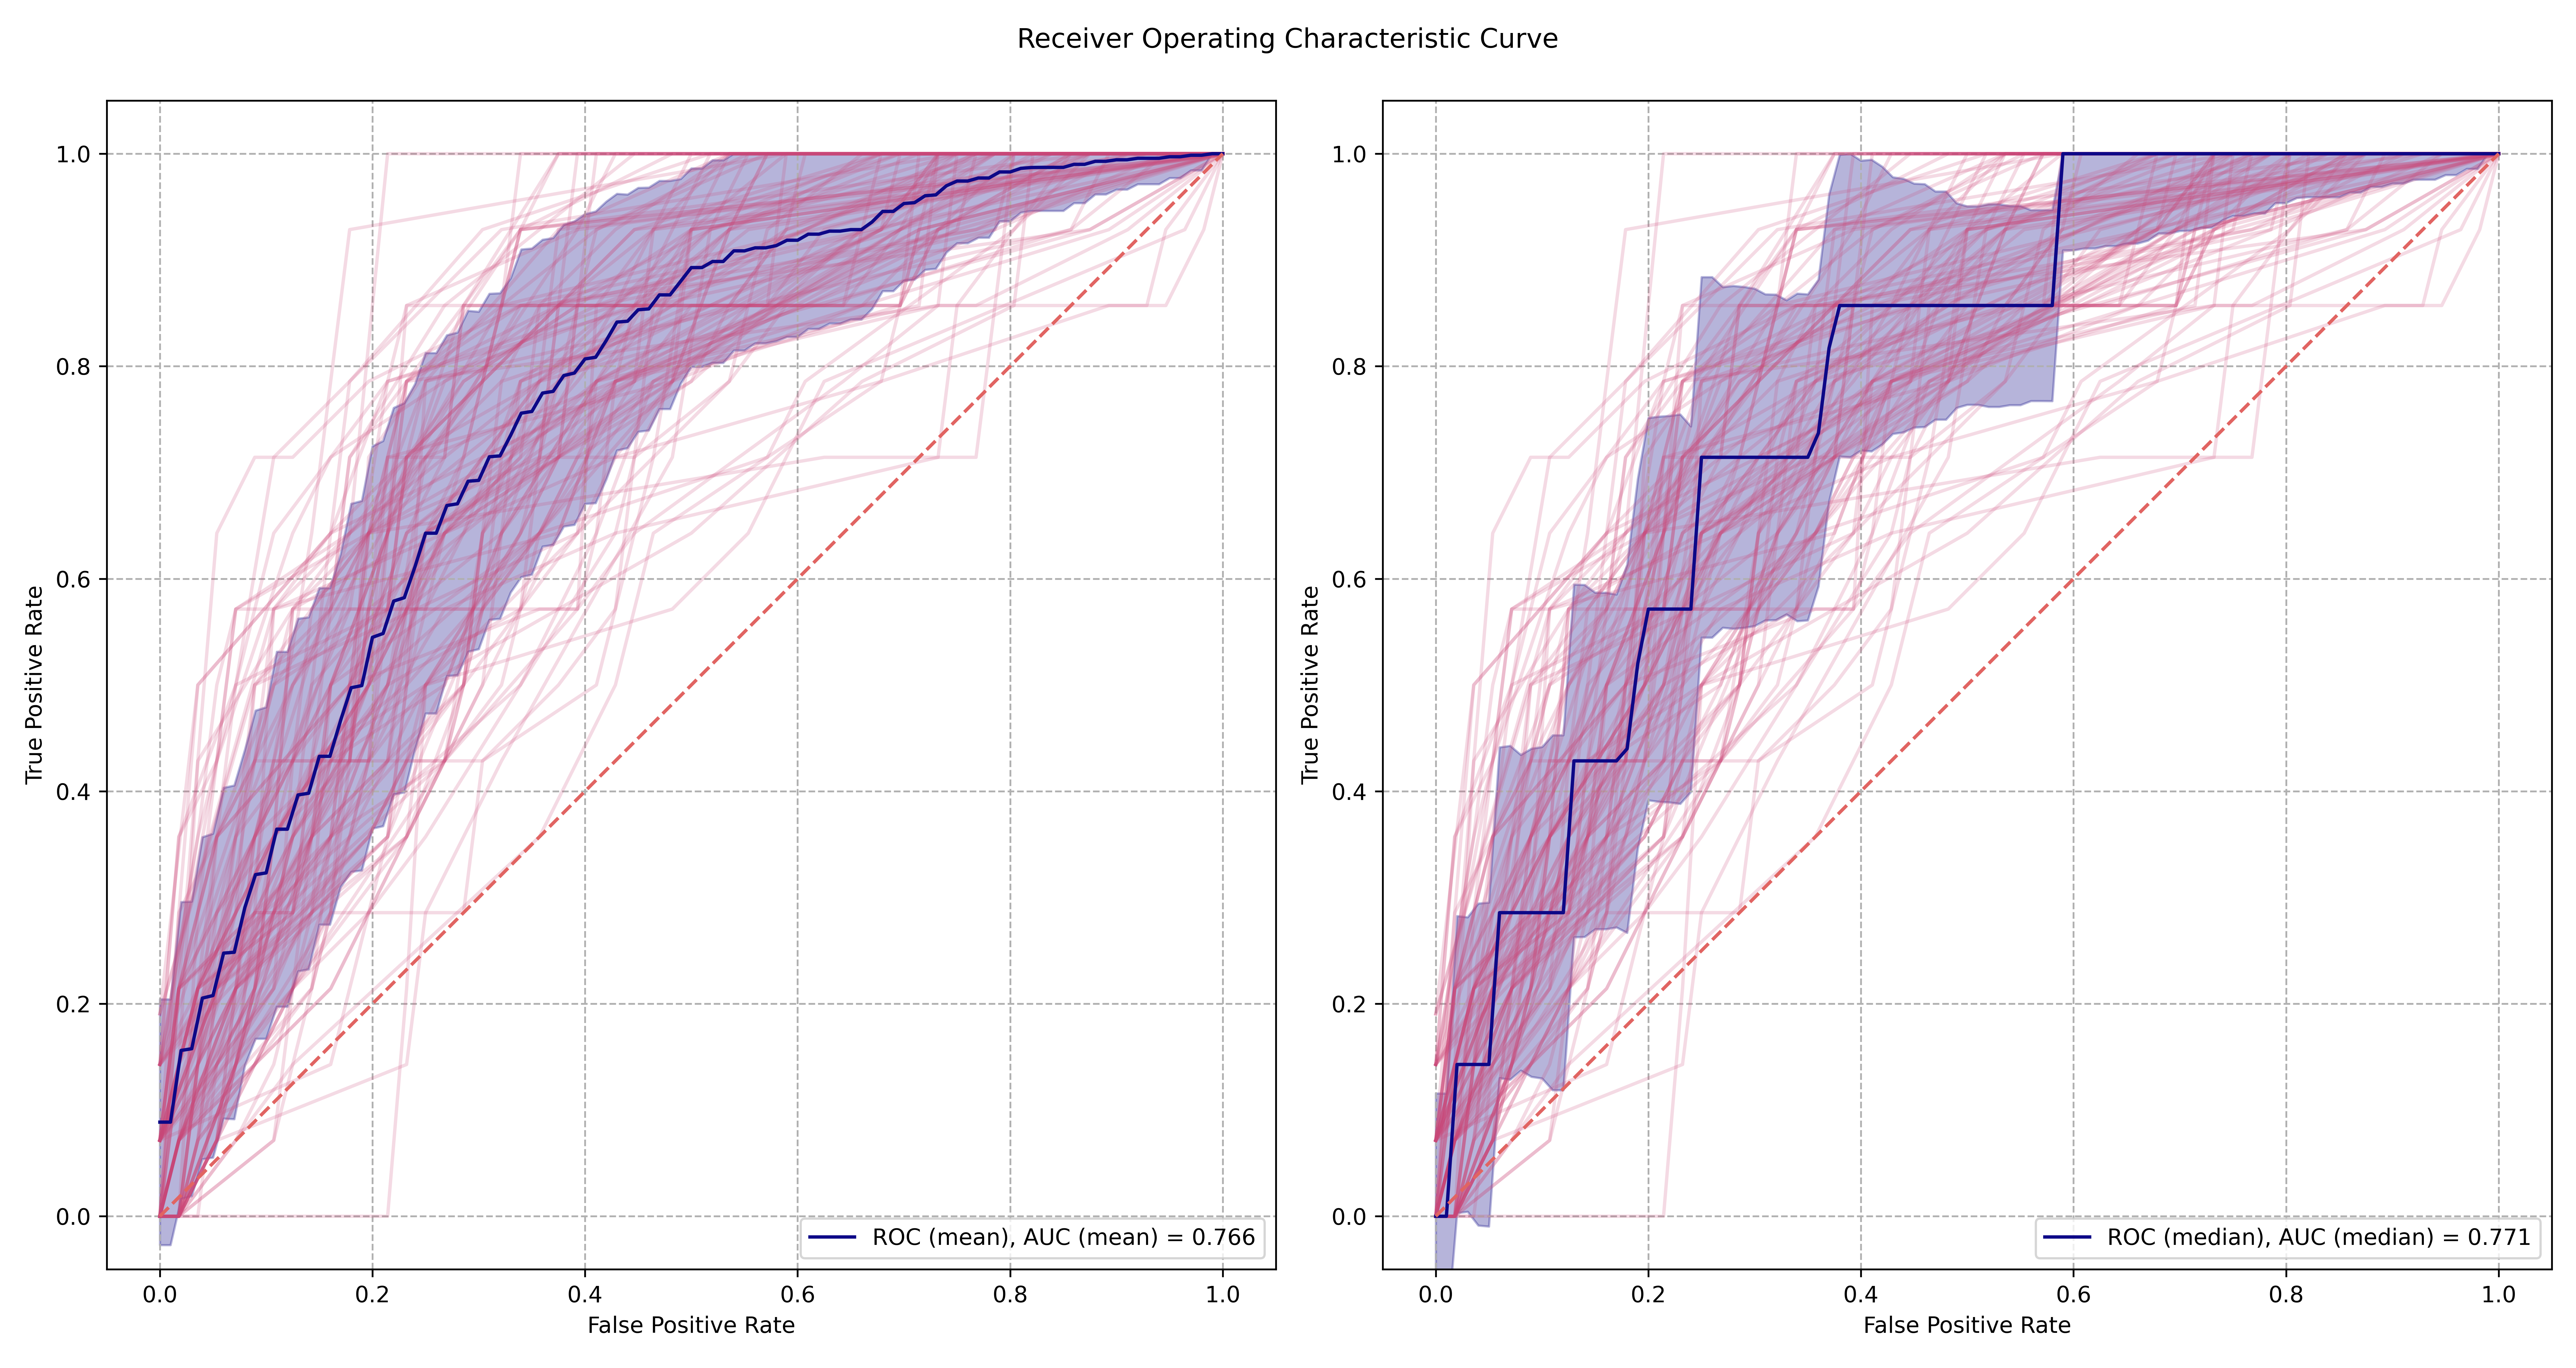
\includegraphics[width=\textwidth]{img/avg_roc.png}
    \caption{\ac{roc} curves for an importance filter level of \num{2.17280844256e-4}. Darker curves show the average, while the shading denotes standard deviation. Semitransparent curves show individual \acp{roc}.}\label{fig:avg_roc}
\end{figure}

% \subsection{Feature Grouping}

While features were treated as a single, all-containing set in the above 
classifications, grouping features shows clear differences in the effect of 
individual feature groups on a successful classification. \enquote{Synergy}
inside a grouping was measured by the ratio of the balanced accuracy the model
trained on that group reached (evaluated over 100 instances) to the average of
importance of features in that group. The importance was measured as described 
in Section~\ref{sec:filtering_importance}, comparing features against all 
available. Groupings deemed \enquote{synergetic} were those that achieved 
unusually high synergy. As expectations about differences in these synergy 
levels were unclear, an arbitrary condition has been chosen; synergy is 
\enquote{unusual} if lies outside the \SI{95}{\percent} confidence interval of
a linear regression over all groupings of the same category. It must be noted 
that there are grounds to suspect this methodology is flawed, as discussed in 
Section~\ref{sec:discussion}. Outlier groupings can be seen in 
Figure~\ref{fig:accuracy_vs_importance}, sitting outside the shaded area marking
the confidence interval.

\begin{figure}[H]
    \centering
    \makebox[\textwidth][c]{\includegraphics[width=1.15\textwidth]{img/accuracy_vs_importance.png}}
    \caption{The balanced accuracy per feature grouping in relation to that grouping's average importance per feature. Larger dots denote larger groups. The line represents a linear regression, with the lightly shaded area marking the \SI{95}{\percent} confidence interval. Groupings that fall outside the confidence interval are labelled in \textit{italics}. Labels for feature method groups have been omitted in favor of legibility. The full information these plots are based on can be found in the appendix under Section~\ref{sec:accuracy_vs_importance}.}\label{fig:accuracy_vs_importance}
\end{figure}



% TODO: Analyze the results further

% Plot Group Performance vs Avg Importance

%  Good    /  o
%      o  o
%        /   o
%   o   / o
%      /  o
%     / o  o Bad
% /\ Group performance
% -> Avg Importance


% Generate and plot AUC/ROC for best accuracy
\newpage{}
\section{Discussion}\label{sec:discussion}

This thesis has shown the construction and evaluation of \iac{rf}-based 
machine learning classifier for the prediction of \ac{pcr} in colorectal 
tumor patients. Considering the performance of this classifier, the 
prediction of \ac{pcr} through \ac{mri}-based radiomics features seems, on 
average, possible.

The assignment of a weighted average of importance to individual features helped
to improve the model. It must be considered that, as the testing set was involved in the selection of
features, results generated through the classification of this set may present
a biased evaluation of the total model performance. Due to its involvement in 
feature filtering, testing data was not completely \enquote{unknown} during the
construction of the classifier model. This suggests, that a more 
representative model accuracy can be obtained using a training/validation/test 
set split, as to not weigh feature selection in favor of a \enquote{known} 
test set~\cite{fundamentals_of_machine_learning}.

Although the usage of importance-based filtering raised the overall accuracy, the relation
between filter levels and model performance did not conform to 
expectations. As stated in Section~\ref{sec:hypothesis}, filtering by importance
was thought to immediately improve accuracy, as a large amount of unnecessary
or non-discriminative features was removed from the dataset. Instead, performance
climbed only with higher filter levels. Although more features were dropped than
initially expected, the number of features used is still significantly higher 
than in comparable studies. The filter level for optimal balanced accuracy 
leaves a set of 329 features, compared to the 30 identifiers used 
in~\cite{radiomics_analysis_pcr_rectal}, 18 used in~\cite{rectal_radiomics_svm_rf} 
and 4 used in~\cite{multisite_rectal_radiomics}. % TODO: Check this!!!!!!!!!1
As two of these studies~\cite{radiomics_analysis_pcr_rectal,rectal_radiomics_svm_rf} achieved higher \ac{auc} scores than the model created 
here, both at its best performance and with a significantly smaller feature set,
this may indicate the usage of a flawed feature selection method.
It must be noted, that both of these studies relied on classification methods,
that do not match \iac{rf} model exactly. When taking into consideration the
study with a matching classifier model,~\cite{multisite_rectal_radiomics}, a
similar \ac{auc} score was achieved\footnote{The classification scores for the model
presented in this thesis is a composite value. In a single model instance, both
better and worse results are possible.}, which calls this conclusion 
into question.

Another conflict arises in the determination of importances used here when 
compared to the performance of grouping-based models. Initially, it was assumed
that these metrics share a positive covariance, that is, a group of features 
deemed more important on average is expected to perform better together. 
If a linear relationship is assumed, the simple linear regression describing 
this relationship, as seen in Figure~\ref{fig:accuracy_vs_importance}, calls this
into question. While an equal number of positive and negative correlations show
up, none are statistically significant. 

Two possible conclusions are drawn here to possibly explain this unexpected 
behavior. Firstly, the metric of importance, as defined in the context of this
thesis, may not accurately describe how individual features contribute to the 
final result. An argument against this is posed by the improvement to model 
performance caused by importance-based filtering. Still, this improvement is not
proven to arise solely (or mostly) from the removal of less important features,
rather than from the reduction of features in general. The latter could be argued using
the conclusion of~\cite{considerations_of_sample_and_feature_size}, which 
states that an abundance in features in relation to training cases can 
negatively affect model performance.

Secondly, the possibility of an ill-fitting analysis. The connection between
group importance may exist, but not be accurately characterized by a simple 
linear regression. This would imply the necessity of using either 
non-linear regression or a more careful examination of outliers. Although this
circumstance is believed to be possible, its further exploration has been 
intentionally omitted in order to avoid accidental cherry-picking.

Having taken possible weaknesses of the metric defined in 
Section~\ref{sec:filtering_grouping} and used in the analysis of 
Figure~\ref{fig:accuracy_vs_importance} into consideration, its results may 
still be of interest in the classification of \ac{mri} imaging data.
When grouping features by the filter applied to the original imaging data, 
\enquote{\acp{lbp}} consistently achieve unexpectedly high synergy, both when measured by
mean and median importance. This is consistent with~\cite{local_binary_patterns},
which introduced this metric as a tool for the analysis of tissue texture.
Other filters such as \enquote{gradient} and \enquote{\ac{log}} achieved high synergy in either mean
or median importance analysis, but failed to reproduce this result in the other.
Wavelet filters, describing spatial frequencies across the input image, showed
consistently high synergy for \enquote{HLL}. Other wavelet configurations 
achieved unremarkable or even very low synergy. The only filters consistently 
resulting in a remarkably low synergy are \enquote{logarithm} and \enquote{squareroot}, along with 
the \enquote{original}, unfiltered image data.

When combining features by their respective feature group, as defined by 
PyRadiomics~\cite{py_rad}, the only groupings to stand out are \enquote{\ac{glrlm}}
and \enquote{shape}, performing better and worse than expected in one 
averaging category respectively. The low synergy in spite of high average 
importance in the \enquote{shape} group may indicate redundant information 
between members of that group. If so, individual features may achieve a high
importance on their own, but do worse than expected in combination. Should this
be true, it calls the effectiveness of the annotation interpolation algorithm
used in this thesis (see Section~\ref{sec:3d_and_2d}) into question.

Both because of this category's large amount of groups and of the regression's
comparatively small confidence interval, grouping by feature extraction method
shows an unusual amount of outliers. In fact, the vast majority of available 
groupings, measured by both mean and median importance, are outliers, with 
80 and 76 groupings out of a total of 99 respectively. Generally, outliers
above the confidence interval largely consist of texture-based features, 
agreeing in part with the earlier groupings categories. In general, texture
features appear to be important for successful classification, both in agreement
with the findings of this thesis and with earlier works~\cite{rectal_radiomics_svm_rf,radiomics_analysis_pcr_rectal}.
In contrast, shape-based
features dominate positions of high average importance but low synergy. This
 may lead to the assumption, that these features do not hold relevant 
information for classification. It must be considered though, that due to 
the non-existence of annotation-based filters, these groups largely consist of
a single feature. 

The grouping of features by category has shown groupings of both high accuracy
and high synergy. Though no grouping has achieved better accuracy than the 
overall model, as described in Section~\ref{sec:filtering_importance}, groupings
like \enquote{lbp-3D-m1} or \enquote{ZonePercentage} show significant performance with both a smaller 
feature count and low assigned \enquote{importance}. This may indicate the 
possibility of higher model accuracy and improved build duration through the
choice of a more rigorous feature selection method.

Overall, a model that, on average, successfully predicts \ac{pcr} has been 
constructed. Although techniques to improve model accuracy have been 
implemented, their exact effects are not yet fully understood and require further 
investigation.

% Write about (un)expected importance/accuracy (in-)coherence

% TODO: Go over bib.bib. Make sure titles are enclosed in {}

\newpage{}